\chapter{Using a CNN to solve the Problem}
\label{ch:solution}

\section{Basic Model Structure}

As it is one of the most conventional approaches, we tried using a convolutional neural network built in \texttt{Tensorflow} \cite{tensorflow} to classify the images.
This, while not overly creative, seemed to be the safest approach to get good results. \\

Considering the amount of data available to us and that the dataset is indeed quite balanced, we chose accuracy as our metric.
We arbitrarily chose a set of parameters for the network, so that, once we had a relatively well-working model,
we could start optimising the hyperparameters. \\

As the input data were coloured images of size $256 \times 256$, we set the input shape to $(256, 256, 3)$.
The first model we used consisted of three convolutional layers with an ascending number of filters, to capture ever more complex features, 
each followed by a max-pooling layer before a flattened fully connected layer which in turn was followed by two dropout layers.
The exact structure can be seen in \autoref{fig:initial_model}. \\

\begin{figure}[H]
    \centering
    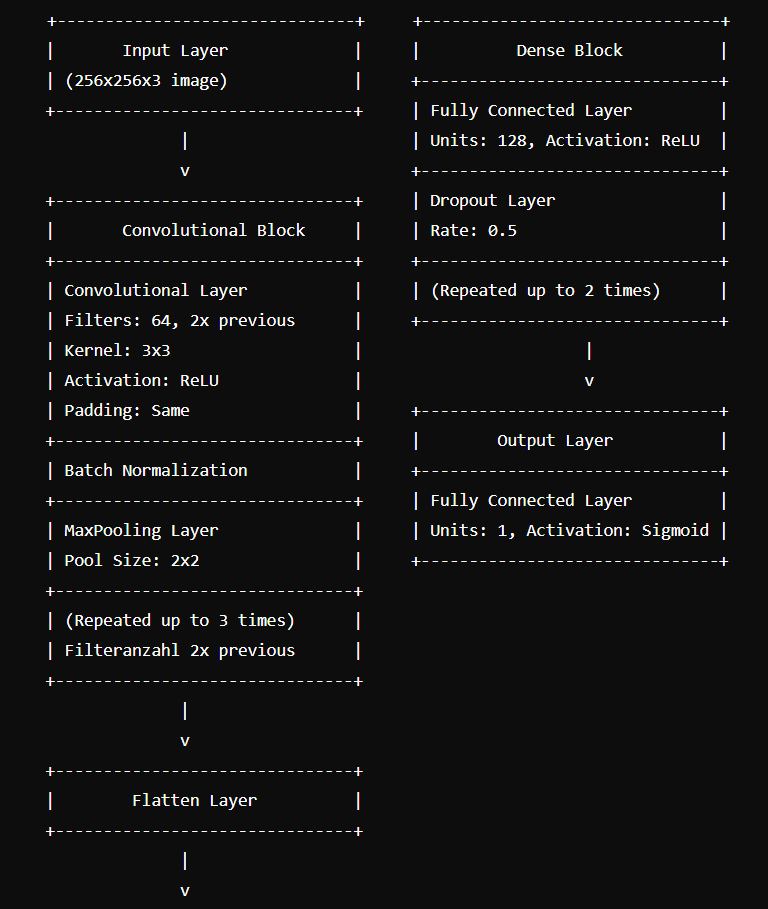
\includegraphics[width=0.5\textwidth]{images/initial_model.png}
    \caption{Structure of the initial model.}
    \label{fig:initial_model}
\end{figure}

While we considered whether a model with three layers was too powerful for the task at hand, we still wanted to test it out.
The increasing number of filters was chosen in order to allow the network to learn more complex features deeper into the model,
with the max-pooling layers picking out the most prominent features.
From the start, we tried avoiding overfitting as much as possible, thus the dropout layers and the L2-regulariser.
The dropout we chose was in the region of around $50 \,\%$, as it seemed inefficient to throw away even more weights and insufficient to choose a lower dropout. \\

After each layer, we normalised the data using batch normalisation, hoping this would cut down on the rather substantial training time, while keeping stability.
We used the ReLU activation function for the convolutional layers and the sigmoid function for the output layer, with adam as the optimiser used to compile the model.
Again, these are the most common choices, with the adam optimiser drastically cutting down on training time, 
while the activation function was later used as a part of the hyperparameter optimisation.
In a further effort to save time, we utilised \texttt{EarlyStopping} to stop the learning process early if the model did not improve for a certain number of epochs
and \texttt{ReduceLROnPlateau}, which reduced the learning rate if necessary, both from the \texttt{keras.callback} library \cite{keras}.
The loss was calculated using binary cross-entropy.  \\

And while is not yet time to talk about the results in depth, this did in fact not exactly produce the results we hoped it would.
Even though the accuracy was quite high at around $95 \,\%$, a closer look at the loss and accuracy curves showed that the model was greatly unstable
with jumps of over $20 \,\%$ in accuracy between epochs.


\section{A First Hyperparameter Optimisation}
\label{sec:results}

We still decided to perform a simple grid search, hoping that the instability arose from simply a poor choice of parameters.
The parameters we chose to optimise were the number of convolutional layers as well as the \texttt{max\_filters} within them, the dropout rate, the number of dense nodes
and the activation function.
Changing the learning rate did not seem necessary as, at the time, we used an adaptive learning rate in our model. 
Shown in \autoref{tab:hyperparameters} are the different parameter values used in the grid search. \\

\begin{table}[H]
    \centering
    \begin{tabular}{ll}
        \toprule
        \textbf{Hyperparameter} & \textbf{Chosen Values} \\
        \midrule
        Number of convolutional layers               & {$2, 3$}\\
        Maximum number of filters                    & {$32, 64, 128$}\\
        Dropout rate                                 & {$0.4, 0.5$}\\
        Number of nodes in dense layers              & {$128, 256, 512$}\\
        Activation function for convolutional layers & {LeakyReLU, ReLU}\\
        Total number of combinations                 & $72$\\
        \bottomrule
    \end{tabular}
    \caption{Chosen Hyperparameters for Model Optimization}
    \label{tab:hyperparameters}
\end{table}

\begin{table}[H]
    \centering
    \caption{The ten best combinations of hyperparameters for the first approach.}
    \label{tab:hyperparameter_optimisation_1}
    \resizebox{\textwidth}{!}{%
    \begin{tabular}{|c|c|c|c|c|c|c|c|c|c|}
        \hline
        \textbf{num\_conv\_layers} & \textbf{max\_filters} & \textbf{dropout} & \textbf{dense\_nodes} & \textbf{activation\_function\_conv} & \textbf{best\_val\_acc\_train\_acc} & \textbf{best\_val\_acc} & \textbf{best\_val\_acc\_train\_loss} & \textbf{best\_val\_acc\_loss} \\
        \hline
        3 & 64  & 0.5 & 128 & ReLU      & 0.950067 & 0.94170 & 0.148508 & 0.187000 \\
        \hline
        3 & 64  & 0.5 & 512 & ReLU      & 0.943667 & 0.93470 & 0.146905 & 0.170992 \\
        \hline
        3 & 32  & 0.4 & 128 & ReLU      & 0.945200 & 0.93450 & 0.144197 & 0.176641 \\
        \hline
        3 & 64  & 0.5 & 256 & ReLU      & 0.934067 & 0.93260 & 0.180251 & 0.190638 \\
        \hline
        3 & 64  & 0.4 & 256 & ReLU      & 0.948133 & 0.93255 & 0.166233 & 0.231369 \\
        \hline
        3 & 32  & 0.4 & 256 & ReLU      & 0.939467 & 0.93235 & 0.152721 & 0.172946 \\
        \hline
        3 & 128 & 0.5 & 256 & ReLU      & 0.942233 & 0.93210 & 0.170646 & 0.220632 \\
        \hline
        3 & 32  & 0.5 & 128 & ReLU      & 0.944000 & 0.93205 & 0.152347 & 0.175270 \\
        \hline
        3 & 32  & 0.5 & 512 & ReLU      & 0.940367 & 0.93100 & 0.188370 & 0.220867 \\
        \hline
        3 & 32  & 0.5 & 128 & LeakyReLU & 0.939433 & 0.93100 & 0.162308 & 0.175924 \\
        \hline
        3 & 32  & 0.4 & 512 & ReLU      & 0.936833 & 0.93065 & 0.159870 & 0.176201 \\
        \hline
    \end{tabular}}
\end{table}

Here, we encountered another problem: this selection of parameters was already very limited and yet took multiple days to compute even though we
had already reduced the image size to $128 \times 128$ pixels.
While the general accuracy was in fact quite high, as can be seen in \autoref{tab:hyperparameter_optimisation_1},
the same instability, if not worse most of the time, could still be seen when taking a look at the accuracy and loss curves.
Still, the model did not necessarily appear to be overfitting, meaning we could still learn something from the hyperparameter optimisation.
The best combinations generally consisted of the models with three convolutional layers and ReLU as the activation function.
Also, a dropout rate of $0.5$ seemed to perform minutely better, although it is hard to say for sure. \\

We concluded that the instability did not come from a poor choice of parameters but instead hinted at a more fundamental problem in our model.
This lead us to adapt our approach, but even with fewer layers, and without batch normalisation, the problem persisted.
As the activation function was also already changed during our hyperparameter optimisation, this didn't seem to be the cause of our problem either.
After more consideration, we arrived at three possible solutions to our problem: we could either lower the learning rate even more, train our model using cross-validation,
or try building our model on top of a model that was already trained on a large amount of images.
As the first two options would have taken a lot of training time, which already was very high, especially concerning the hyperparameter optimisation,
we decided to go with the third option.
Although unsatisfying, it was the only viable choice. \\

The pre-trained model we picked was the \texttt{VGG16}-model \cite{VGG16source}, which is a very deep convolutional model that was trained on the ImageNet dataset
and we built our model on top of it. \\

This finally yielded satisfying results.


\section{A Second Hyperparameter Optimisation}

In order to obtain the best results with the \texttt{VGG16}-model as a base, we settled on a combination of the best few parameters from the first hyperparameter optimisation
and additionally added the number of dense layers to the list of parameters.
In total, we only checked six different combinations of hyperparameters, as we were quite certain that the previous model was not too far off and frankly out of lack of time.
This list of hyperparameters can be seen in \autoref{fig:VGG16_hyperparameter_optimisation}.

\begin{table}[H]
    \centering
    \caption{The six combinations of hyperparameters for the second approach using the \texttt{VGG16} base model with their respective metrics.}
    \label{tab:VGG16_hyperparameter_optimisation}
    \resizebox{\textwidth}{!}{%
    \begin{tabular}{|c|c|c|c|c|c|c|c|}
    \hline
    num\_conv\_layers & max\_filters & dropout & dense\_nodes & num\_dense\_layers & best\_val\_acc & best\_val\_acc\_loss & F1-Score \\
    \hline
    3 & 256 & 0.5 & 128 & 1 & 0.96550 & 0.094746 & 0.975520 \\
    3 & 128 & 0.5 & 256 & 1 & 0.95955 & 0.112311 & 0.973051 \\
    3 & 128 & 0.5 & 256 & 2 & 0.95930 & 0.114798 & 0.972138 \\
    3 & 128 & 0.5 & 128 & 1 & 0.95975 & 0.108166 & 0.970034 \\
    3 & 128 & 0.5 & 128 & 2 & 0.96005 & 0.111835 & 0.969091 \\
    3 & 256 & 0.5 & 256 & 1 & 0.95745 & 0.118781 & 0.968652 \\
    \hline
    \end{tabular}}
\end{table}
\begin{figure}[H]
    \centering
    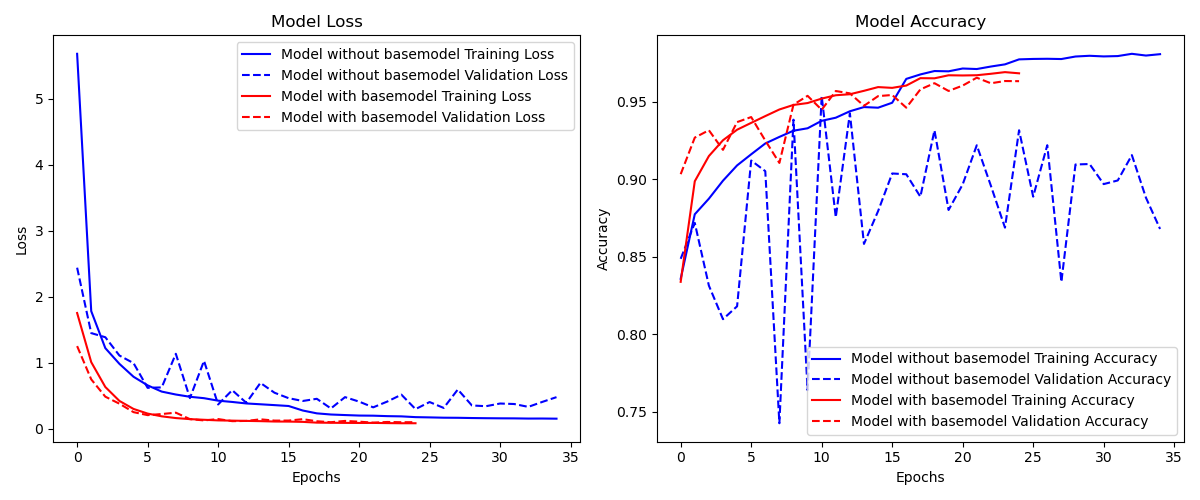
\includegraphics[width=\textwidth]{images/VGG16_best_parameters_comparison.png}
    \caption{Training and Validation loss and accuracy for the best sets of hyperparameters for both the first model and the model built atop \texttt{VGG16}.
    The blue curves represent the first model, while the red curves represent the model built using the \texttt{VGG16} base model.}
    \label{fig:VGG16_hyperparameter_optimisation}
\end{figure}

The first thing to be noted here is that the accuracy is visibly higher than before, with the best model reaching an accuracy of almost $97 \%$.
This time, we also included the F1-score and recall in our evaluation, hoping to spot possible problems concerning stability earlier.
Further, the issue of instability was also resolved.
This can be seen in \autoref{fig:VGG16_hyperparameter_optimisation}, which also emphasises the stark difference in stability between the first and the adapted model.

While at the beginning, there still is a slight instability, the validation accuracy now nicely converges against the training accuracy.
It should also be remembered that this hyperparameter optimisation was done with all weights of the \texttt{VGG16}-model frozen,
meaning that on the model we built on top was actually trained on the dataset.
The impact of the number of trainable layers in the \texttt{VGG16}-model can be seen in \autoref{fig:VGG16_comparison}.

\begin{figure}[H]
    \centering
    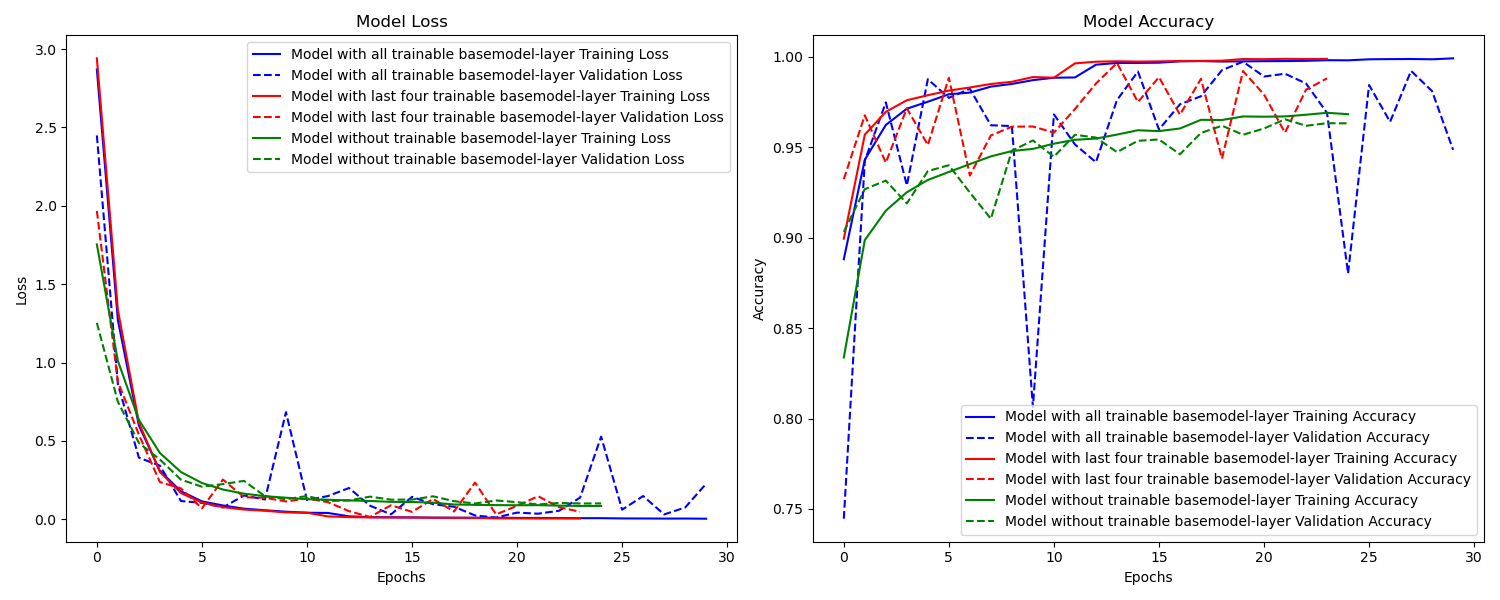
\includegraphics[width=\textwidth]{images/VGG16_comparison.png}
    \caption{Comparison of the validation accuracy and loss between the models with different numbers of trainable layers.
    The green curve shows the frozen base model, while the red curve shows a version where the last four layers were trained and blue curve the model with all layers trainable.}
    \label{fig:VGG16_comparison}
\end{figure}

This clearly shows the trade-off between accuracy and stability.
As the number of trainable layers increases, so does the accuracy, but the meticulously created stability is lost again.
The best compromise between stability and accuracy was found with the model where only the last four layers were trained, 
as its accuracy is only slightly lower than the model where all layers were trained, but the stability is much higher.



